 \begin{center}
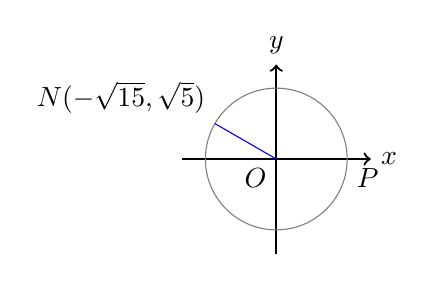
\begin{tikzpicture}[scale=0.6]
\draw[->, thick](-2,0)--(2,0)node[anchor=west]{$x$};
\draw[->, thick](0,-2)--(0,2)node[anchor=south]{$y$};
\draw[gray](0,0)circle(1.5);
\draw[draw=blue](0,0)node[anchor=north east]{$O$} -- (150:1.5)node[anchor=south east]{$N (-\sqrt{15},\sqrt{5})$};
\draw(1.5,0)node[anchor=north west]{$P$};
\end{tikzpicture}\end{center}
In the $xy$-plane above, $O$ is the center of the circle, and the measure of $\angle NOP$ is $\theta\pi$ radians.  What is the value of $\theta$?\\ \\


\ifsat
	\begin{enumerate}[label=\Alph*)]
	\end{enumerate}
\else
\fi

\ifacteven
	\begin{enumerate}[label=\textbf{\Alph*.},itemsep=\fill,align=left]
		\setcounter{enumii}{5}
		\item None of these. 
	\end{enumerate}
\else
\fi

\ifactodd
	\begin{enumerate}[label=\textbf{\Alph*.},itemsep=\fill,align=left]
		\item None of these. 
	\end{enumerate}
\else
\fi

\ifgridin
$\frac{5}{6}$ or $.833$
\else
\fi

